%HEPATITIS SLIDES
\begin{frame}
\frametitle{How important is HCV?}

\begin{columns}[t]

\column{.5\textwidth}

\footnotesize{
\begin{itemize}
	\item 170m+ infected
	\item ~80\% infections are chronic
	\item Liver cirrhosis \& cancer risk
	\item 12,000 deaths per year in USA
	\item No protective immunity?
\end{itemize}
}


\includegraphics[width=0.6\textwidth]{../../images/Cover}

\column{.5\textwidth}

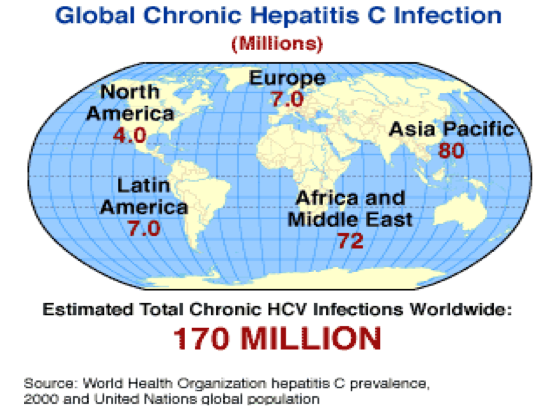
\includegraphics[width=\textwidth]{../../images/GlobeHCV}

\end{columns}

\end{frame}

%Slide45
\begin{frame}
\frametitle{HCV Transmission}
 
\textbf{Percutaneous exposure to infected blood}

\begin{columns}[t]

\column{.5\textwidth}

\begin{itemize}
	\item Blood transfusion / blood products
	\item Injecting \& nasal drug use
	\item Sexual \& vertical transmission
	\item Unsafe injections
	\item Unidentified routes
\end{itemize}

\column{.5\textwidth}

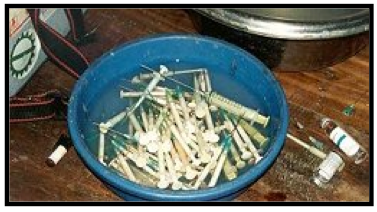
\includegraphics[width=\textwidth]{../../images/Needles}

\end{columns}

\end{frame}

%Slide46
\begin{frame}
\frametitle{Estimating demographic history of HCV using the coalescent}

\begin{columns}[t]

\column{.5\textwidth}

\scriptsize{
\begin{itemize}
	\item Egyptian HCV gene sequences
	\item n=61
	\item E1 gene, 411bp
	\item All sequence contemporaneous
	\item Egypt has highest prevalence of HCV worldwide (10-20\%)
	\item But low prevalence in neighbouring states
	\item Why is Egypt so seriously affected?
	\item Parenteral antischistosomal therapy (PAT)
\end{itemize}
}

\column{.5\textwidth}

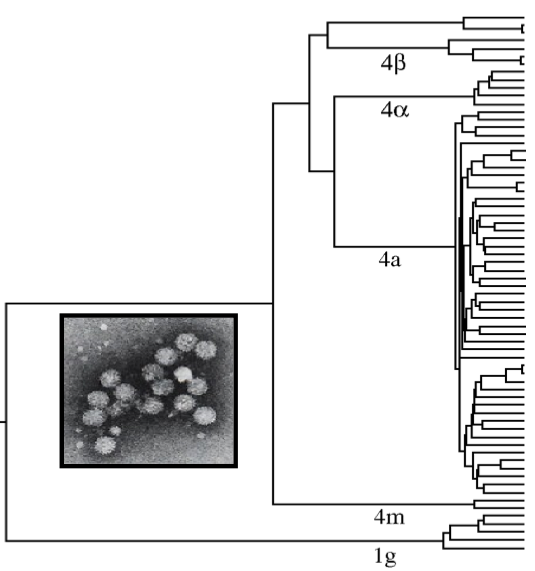
\includegraphics[width=\textwidth]{../../images/HistoryOfHCV}

\end{columns}

\end{frame}

%Slide47
\begin{frame}
\frametitle{Demographic model}

\footnotesize{
\begin{columns}[t]

\column{.5\textwidth}

\begin{itemize}
	\item The coalescent can be extended to model deterministically varying populations.
	\item The model we used was a const-exp-const model.
	\item A Bayesian MCMC method was developed to sample the gene genealogy, the substitution model and demographic function simultaneously.
\end{itemize}

\column{.5\textwidth}

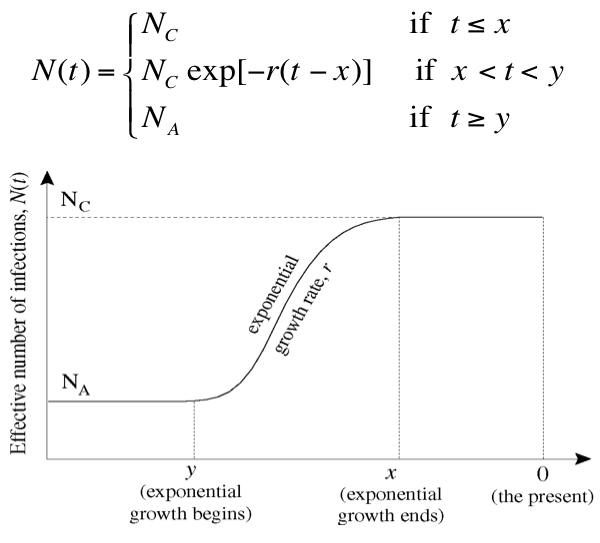
\includegraphics[width=\textwidth]{../../images/DemographicModel}

\end{columns}
}

\end{frame}

%Slide48
\begin{frame}
\frametitle{Estimated demographic history}

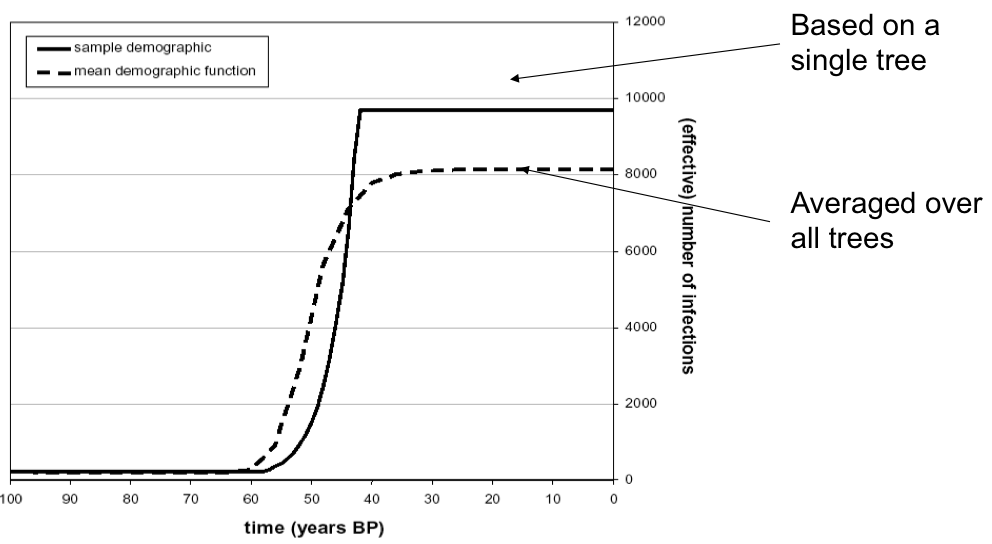
\includegraphics[width=\textwidth]{../../images/DemographicHistory}

\end{frame}

%Slide49
\begin{frame}
\frametitle{Parameter estimates}

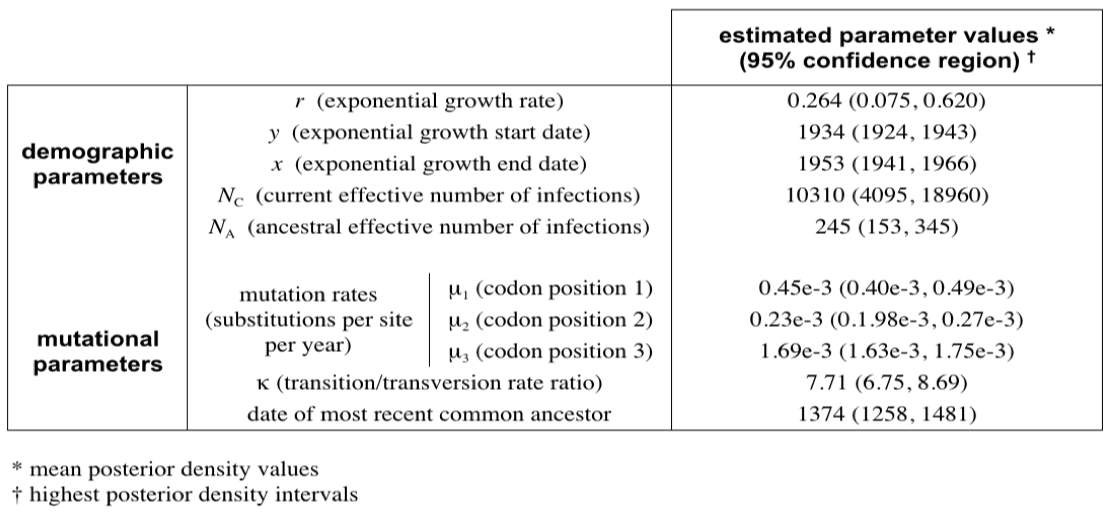
\includegraphics[width=\textwidth]{../../images/ParameterEstimates}

\end{frame}

%Slide50
\begin{frame}
\frametitle{Uncertainty in parameter estimates}

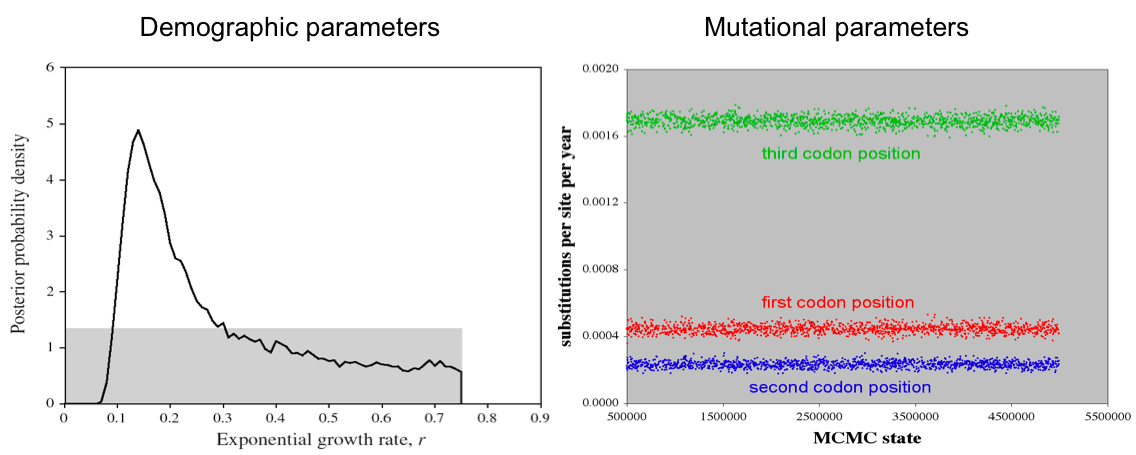
\includegraphics[width=\textwidth]{../../images/UncertaintyParameter}

\footnotesize{
\begin{columns}[t]

\column{.5\textwidth}

Growth rate of the growth phase

Grey box is the prior

\column{.5\textwidth}

Rates at different codon positions,

All significantly different

\end{columns}
}

\end{frame}

\begin{frame}
\frametitle{Full Bayesian Estimation}

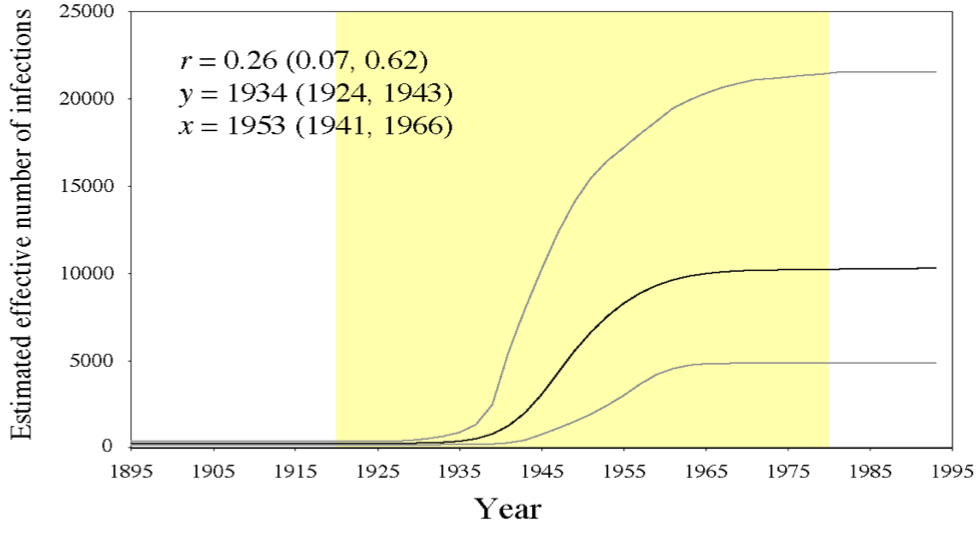
\includegraphics[width=\textwidth]{../../images/FullBayesianEstimation}

\footnotesize{
\begin{itemize}
	\item  Marginalized over uncertainty in genealogy and mutational processes
	\item  Yellow band represents the region over which PAT was employed in Egypt 
\end{itemize}
}

\end{frame}
